\documentclass[a4paper,openright,12pt]{article}
\usepackage[utf8]{inputenc}
\usepackage{geometry}
\usepackage{soul}
\usepackage{mathptmx}
 \geometry{
 a4paper,
 total={170mm,257mm},
 left=25mm,
 right=25mm,
 top=18mm,
 bottom=19mm,
 }
 \usepackage{graphicx}
 \usepackage{titling}
 \usepackage{eurosym}
\usepackage{lipsum}  
\usepackage{listings}
\usepackage[spanish]{babel}
\usepackage{hyperref}
\usepackage{amsmath}
\usepackage{float}

\usepackage{caption}
\usepackage{subcaption}
 
\usepackage{fancyhdr}
\fancypagestyle{plain}{%  the preset of fancyhdr 
    \fancyhf{} % clear all header and footer fields
   % \fancyfoot[R]{
\includegraphics[width=2cm]{UGR_LOGO.png}}
   % \fancyfoot[L]{\thedate}
    \fancyhead[L]{MUIT - Sistemas Electrónicos Integrados}
    \fancyhead[R]{\theauthor}
}



\begin{document}

\begin{titlepage}
 
 
\newlength{\centeroffset}
\setlength{\centeroffset}{-0.5\oddsidemargin}
\addtolength{\centeroffset}{0.5\evensidemargin}
\thispagestyle{empty}

\noindent\hspace*{\centeroffset}\begin{minipage}{\textwidth}

\centering

\includegraphics[width=0.9\textwidth]{imagenes/logo_ugr.jpg}\\[1.4cm]

\textsc{ \Large Proyecto de sistemas electrónicos integrados}\\[1cm]
% Upper part of the page
% 
% Title
{\LARGE \bfseries Diseño de un sistema de captación de señales satelitales NOAA con corrección de efecto Doppler\\
}
\noindent\rule[-1ex]{\textwidth}{3pt}\\[3.5ex]
{\large\bfseries Recepción y procesamiento de imágenes APT.}
\end{minipage}

\vspace{1cm}
\noindent\hspace*{\centeroffset}\begin{minipage}{\textwidth}
\centering

\textbf{Autores}\\ {Andrés Biedma Pérez\\Javier Lobato Martín\\Sergio Zapata Caparrós}\\[2.5ex]
\textbf{Director}\\
{Javier Díaz Alonso}\\[2cm]

\includegraphics[width=0.3\textwidth]{imagenes/etsiit_logo.png}\\[0.1cm]
\textsc{Escuela Técnica Superior de Ingenierías Informática y de Telecomunicación}\\
\textsc{---}\\
Granada, Enero de 2023
\end{minipage}
%\addtolength{\textwidth}{\centeroffset}
%\vspace{\stretch{2}}
\end{titlepage}




\tableofcontents
\newpage

\section{Introducción}

	El objetivo 	de este proyecto es el diseño de un sistema completo de recepción de imágenes de satélites NOAA. El sistema incluye la especificación y fabricación de una antena adaptada a la naturaleza de la señal que se desea recibir, así como el diseño del software que permita tanto la demodulación y obtención de la imagen como la corrección del efecto Doppler sobre la misma. En los siguientes apartados se realizará un análisis de los distintos apartados del proyecto.
	
	\subsection{Estándar APT}
	
	El estándar APT es un sistema analógico de tranmisión de imágenes, introducido en la década de 1960 para su uso en satélites de meteorología. El objetivo del estándar era permitir a los usuarios recibir imágenes meteorológicas usando estaciones de bajo coste. 
	
	La información transmitida está compuesta por dos canales de imágenes, información de sincronización y telemetría, dispuestas en líneas horizontales de 2080 píxeles. La siguiente figura ilustra la disposición de las imágenes:
	
	\begin{figure}[hbtp]
 \centering
 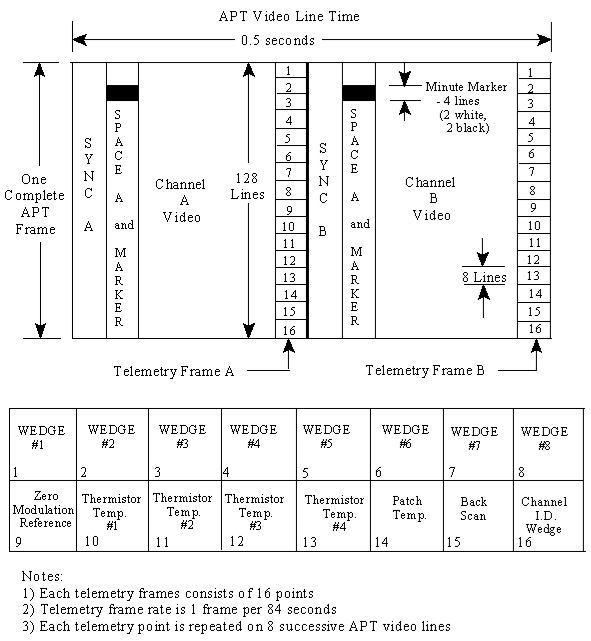
\includegraphics[width = 10cm]{imagenes/APT_frame.JPG}
 \caption{Esquema del estándar APT}
 \label{APT_FRAME}
 \end{figure}


	En concreto, para los satélites NOAA, las imágenes cuentan con una resolución espacial de 4 km/píxel, tomando imágenes del espectro visible e infrarrojo. La información de la imagen se modula AM con 256 niveles de amplitud, para luego modularse en FM en una portadora en la banda de 137 MHz. Esta decisión de modulación permite que con un receptor sencillo se puedan obetener las imágenes que transmite el satélite. La señal es difundida de manera ininterrumpida.

\newpage
	
	
	\subsection{Efecto Doppler}

	El efecto Doppler es un fenómeno consistente en la variación de frecuencia observada por un receptor debido a un movimiento relativo entre emisor y receptor. Para la casuística de satélite-estación receptora, se tiene que el receptor se encuentra estático, y existe cierta velocidad relativa al acercarse y alejarse el satélite al receptor. La consecuencia de este movimiento relativo se traduce en una variación de la frecuencia aparente recibida conforme a la nominal. Este desplazamiento de frecuencia tampoco es constante, ya que la velocidad del satélite con respecto a la estación receptora  no es constante (aunque la velocidad orbital si lo sea). En la demodulación FM se puede hacer frente a este desplazamiento de frecuencia, ya que en el proceso de demodulación es común utilizar elementos como los PLL(Phase-Locked-Loop), que anulan estos efectos. Sin embargo, en la señal AM que contiene la información de la imagen, este efecto sigue presente, y se traduce en una imagen con un aspecto 'doblado', debido a la variación en frecuencia que modifica la longitud efectiva de cada línea. En este proyecto se propondrá un método para la corrección a posteriori de este efecto en las imágenes.

\section{Distribución del proyecto}
El proyecto se ha realizado durante los meses de Diciembre del año 2022 y Enero del año 2023. La distribución del mismo se muestra en la Fig.[\ref{Fig:Gantt}].

\begin{figure}[h!]
    \centering
    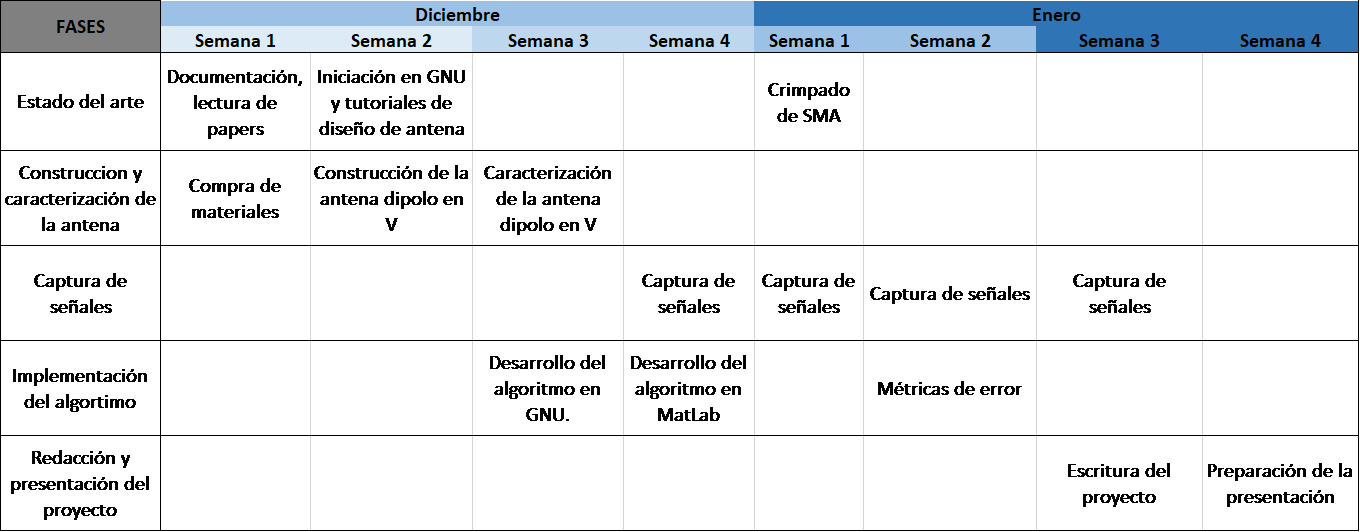
\includegraphics[width=1\linewidth, height=9cm]{imagenes/DiagramaGantt.png}
    \caption{Diagrama de Gantt en el que se recoge la distribución del proyecto.}
    \label{Fig:Gantt}
\end{figure}

Se ha desglosado el trabajo entre los tres integrantes del grupo de trabajo, realizando en paralelo tareas distintas, tanto de hardware como de software, y contribuyendo conjuntamente al objetivo común.

\newpage

\section{Hardware}
Desde el punto de vista del Hardware se ha utilizado una antena tipo dipolo en V y un RTL-SDR, ambos se describen a continuación.
	\subsection{Antena dipolo en V}
 Puesto que se pretende escuchar las imágenes APT transmitida por satélites NOAA, se ha de diseñar una antena que opere en la banda de frecuencia de los mismos, véase Tabla [\ref{Tab1:NOOA_frecuencias}]. 
 \begin{table}[h!]
\centering

\begin{tabular}{|c|c|} 
\hline
\textbf{Satélite} & \begin{tabular}[c]{@{}c@{}}\textbf{Frecuencia}\\\textbf{de emisión [MHz]}\end{tabular}  \\ 
\hline
NOAA - 15           & 137.630                                                                                 \\ 
\hline
NOAA - 18           & 137.9125                                                                                \\ 
\hline
NOAA - 19           & 137.100                                                                                 \\
\hline
\end{tabular}
\caption{Tabla resumen con las frecuencias de emisión APT de cada satélite NOAA.}
\label{Tab1:NOOA_frecuencias}
\end{table}
Además, se ha de tener en cuenta que los satélites transmiten señales RHCP. Si se pretende obtener el mejor rendimiento, es recomendable que la antena seleccionada esté polarizada de acuerdo a RHCP. Dentro de la literatura se encuentran antenas como: antena helicoidal end-fire (\textit{helix antena}), antena helicoidal back-fire (\textit{QFH helix}) o dipolos cruzados, mientras que rara vez se encuentran antenas tipo espiral o \textit{lindelblad} antena, pese a que a priori se pensase en utilizar antenas circulares. Esto se debe a que construir \textit{DIY} antenas con una relación axial igual a 1 (o polarización circular perfecta) resulta realmente difícil y cualquier pequeño error implica: una polarización elíptica y una reducción del ancho de banda de trabajo. 
Es por ello que para elegir la antena que ideal: aquella que se adecuase a nuestras habilidades de construcción y garantizase la recepción de señales procedentes de satélites NOAA, se realizó un análisis de la polarización cruzada, véase Tabla [\ref{Tab2:x_pol}].

\begin{table}[h!]
\centering
\begin{tabular}{|c|c|c|c|c|} 
\hline
\textbf{Polarización} & \textbf{Vertical} & \textbf{Horizontal} & \textbf{RHCP} & \textbf{LHCP}  \\ 
\hline
\textbf{Vertical}     & 0dB               & -20dB               & -3dB          & -3dB           \\ 
\hline
\textbf{Horizontal}   & -20dB             & 0dB                 & -3dB          & -3dB           \\ 
\hline
\textbf{RHCP}         & -3dB              & -3dB                & 0dB           & -20dB          \\ 
\hline
\textbf{LHCP}         & -3dB              & -3dB                & -20dB         & 0dB            \\
\hline
\end{tabular}
\caption{Tabla resumen de la relación de polarización cruzada entre las polarizaciones: vertical, horizontal, LHCP y RHCP.}
\label{Tab2:x_pol}
\end{table}

La tabla \ref{Tab2:x_pol} reafirma lo sensible que puede resultar un error que varíe la polarización en la construcción de la antena. Es por ello que se decidió sacrificar unos cuantos dB y optar por un diseño de antena más simple con polarización lineal. Entre las múltiples ventajas de las antenas de polarización lineal (vertical u horizontal) destacan: la facilidad del diseño, presentan patrones de radiación omnidireccionales, es fácil conseguir una impedancia de antena ($Z_{ant}=50\Omega$), etc.
El detalle que ha hecho que se opte por la polarización horizontal es que la inmensa mayoría de servicios de radio-televisión utilizan polarización vertical y de acuerdo a [\ref{Tab2:x_pol}] esta se ve reducida en -20dB frente a la polarización horizontal. \\

Teniendo en consideración todos los factores mencionados hasta ahora se decidió construir una \textbf{antena tipo dipolo en V} con polarización horizontal que  cumple con las especificaciones requeridas: fácil de construir y funcional en la ancho de banda de trabajo requerido, el único problema que presentan los dipolos son los nulos laterales, sin embargo, este inconveniente se soluciona doblando el dipolo un ángulo $\theta=120º$ de forma que el diagrama de radiación del conjunto de la antena en dirección ortogonal a la misma se vea reforzado. Un modelo 3D de la misma se muestra en Fig.[\ref{fig:modelo3D}], mientras que en Fig.[\ref{fig:topdown}] se muestra la perspectiva top-down.

\begin{figure}[H]
    \centering
    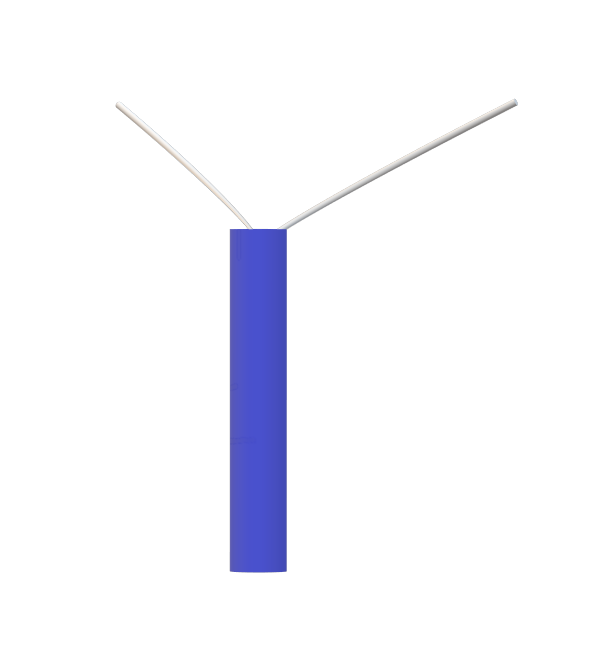
\includegraphics[width=0.45\linewidth]{imagenes/ModeloAntena.png}
    \caption{Modelo 3D de la antena dipolo en V construida.}
    \label{fig:modelo3D}
\end{figure}



Una vez establecida el tipo de antena y la banda de frecuencia de trabajo, se han calculado las medidas de los brazos de la antena de la siguiente forma:

\begin{gather}
        L(m) = 147/f(MHz) \\
       L(m) = 147/137.5 \\
       L(m) = 1.068m = 106.8cm
\end{gather}

Por tanto, cada uno de los brazos ha de medir: 
\begin{equation*}
    L = 53.4cm
\end{equation*}

\begin{figure}[H]
    \centering
    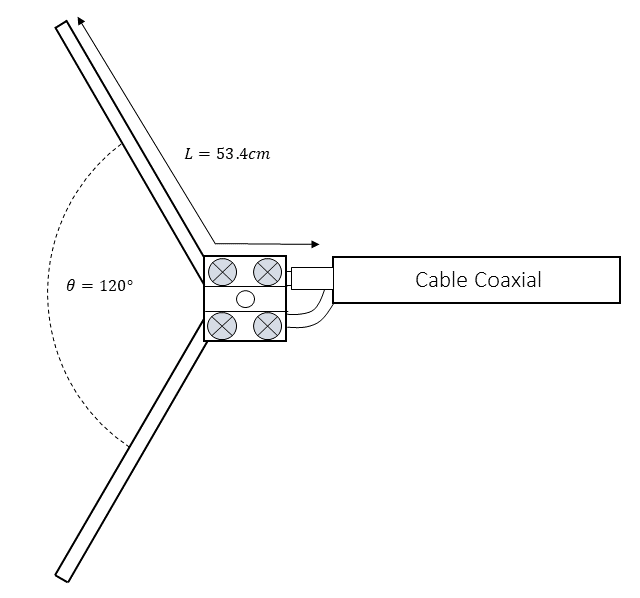
\includegraphics[width=0.5\linewidth]{imagenes/PerspectivaTopDown.png}
    \caption{Perspectiva top-down de la antena dipolo en V construida.}
    \label{fig:topdown}
\end{figure}

Una vez se construyó la antena, se hizo uso de un Vector Network Analyzer (VNA) para comprobar a través del parámetro S11 que la antena se comportaba de acuerdo a lo esperado. Los resultados tras la caracterización de dicho parámetro se muestra en la Fig. [\ref{fig:S11}].
\begin{figure}[H]
    \centering
    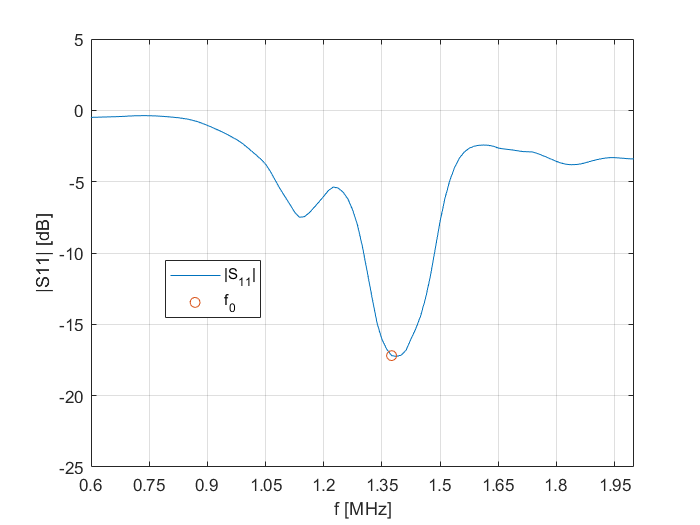
\includegraphics[width=0.55\linewidth]{imagenes/S11.png}
    \caption{Módulo del parámetro S11 medido.}
    \label{fig:S11}
\end{figure}

En la siguiente imagen podemos comprobar el aspecto final de la antena, conectada al dispositivo RTL-SDR y usando la aplicación SDRsharp. La imagen se tomó durante la primera toma de contacto al montar la antena.

\begin{figure}[H]
    \centering
    \includegraphics[width=0.55\linewidth]{imagenes/setup.jpg}
    \caption{Setup de la antena construida, conectada al RTL-SDR y a SDRsharp}
    \label{antena_real}
\end{figure}



	\subsection{RTL-SDR}
	Las siglas SDR (Software Defined Radio) en un sistema de comunicación hacen referencia a la implementación de componentes (tradicionalmente en hardware) por software. En la Figura [\ref{SDR}] se ejemplifica el comportamiento de un SDR.
	
 \begin{figure}[hbtp]
 \centering
 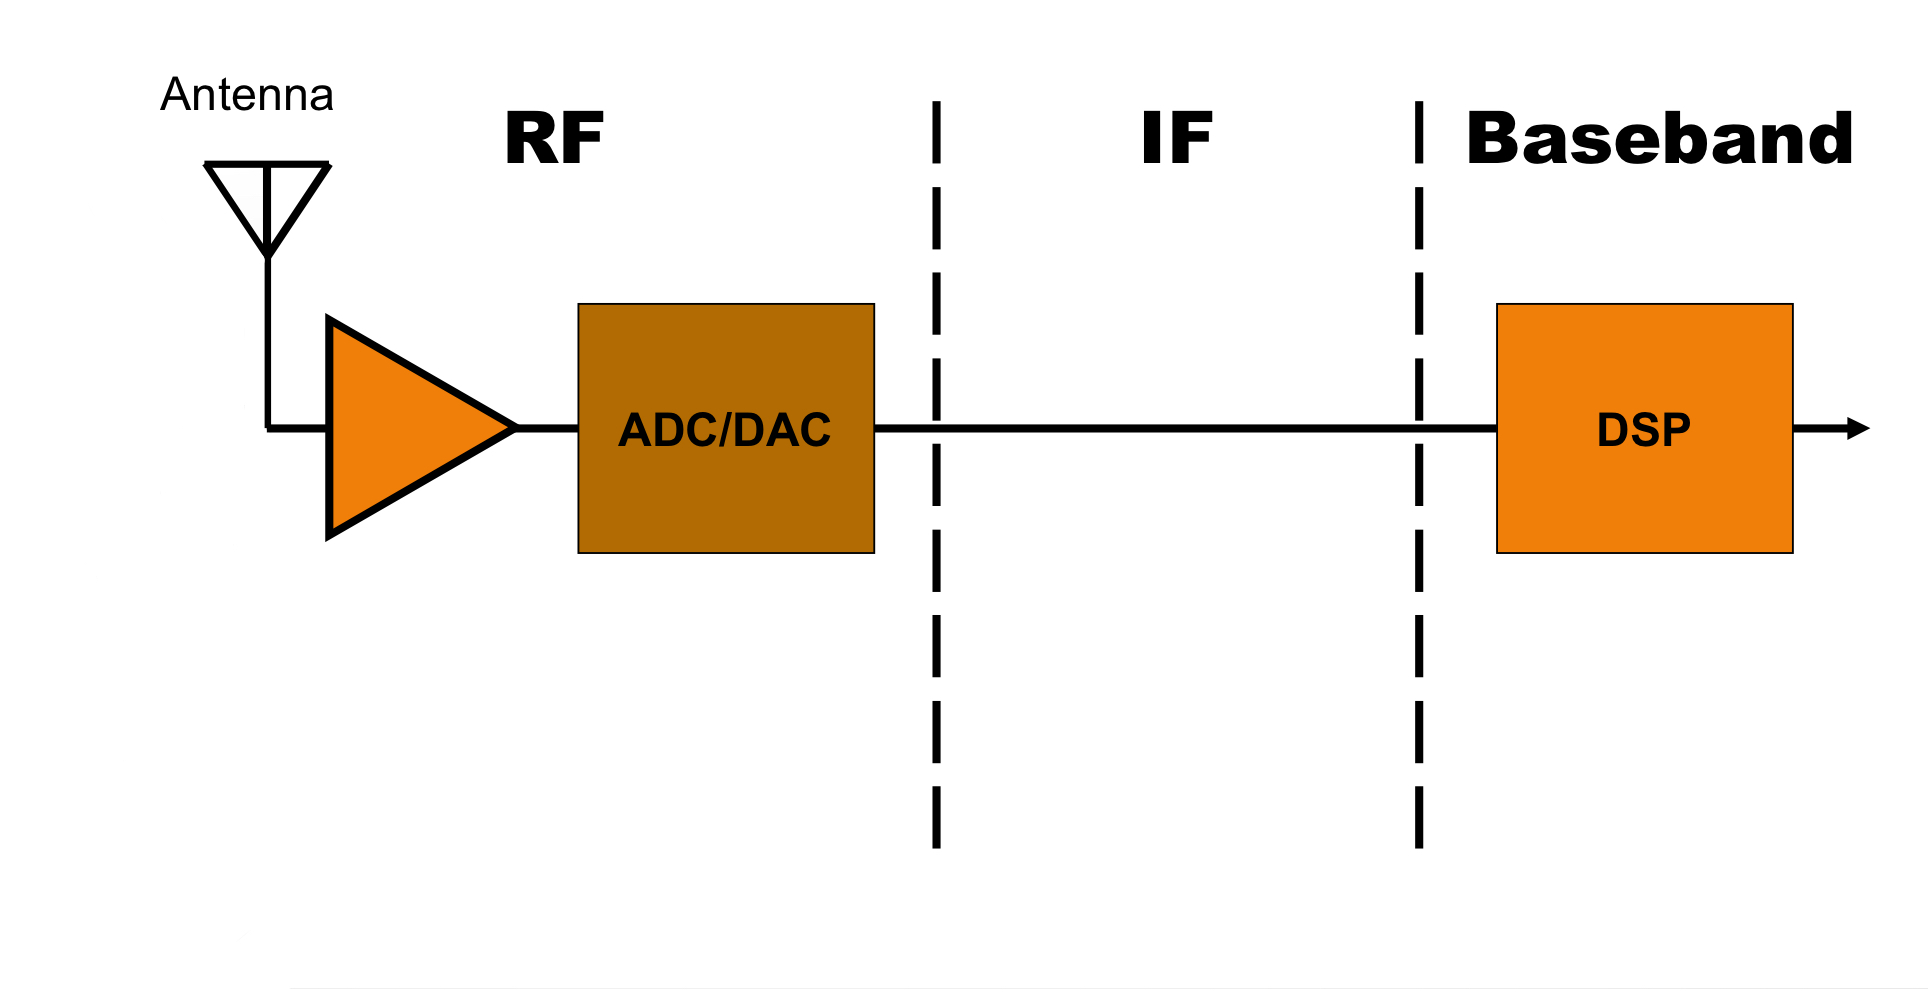
\includegraphics[width = 12cm]{imagenes/sdr.jpg}
 \caption{Software Defined Radio}
 \label{SDR}
 \end{figure}

Directamente se muestrea y se genera la señal en radio frecuencia (RF). Se consigue eliminar la inclusión de componentes en una frecuencia intermedia y se gana en flexibilidad, ya que todo el procedimiento se realiza en el dominio digital. También se obtiene una información más precisa al eliminar posibles mezcladores.

	 En concreto, el dispositivo RTL-SDR es un tipo de radio definida por software a la que se incorpora el chip ''RTL832U''. Este dispositivo es capaz de proporcionar las partes real y compleja de la señal en banda base, pudiendo abarcar gran parte del espectro de radio frecuencia. El sintonizador interno cubre un ancho de banda desde los 25 MHz hasta casi los 2 MHz. La frecuencia máxima de muestreo en este caso se sitúa en $2.4 MHz$.
	 
	 \begin{figure}[H]
  \begin{subfigure}[b]{0.49\textwidth}
    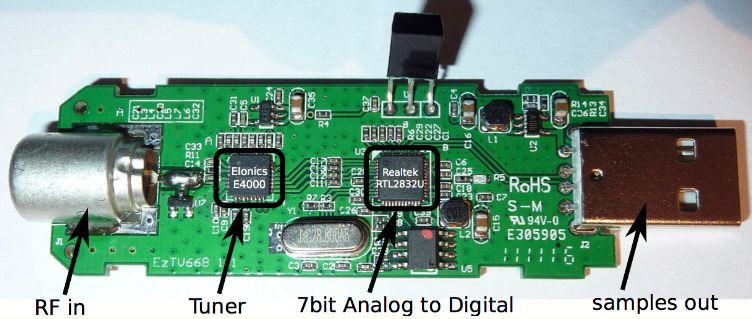
\includegraphics[width=\textwidth, height=5cm]{imagenes/inner_RTL.JPG}
    \caption{Interior RTL-SDR}
    \label{inner_RTL}
  \end{subfigure}
  \hfill
  \begin{subfigure}[b]{0.49\textwidth}
    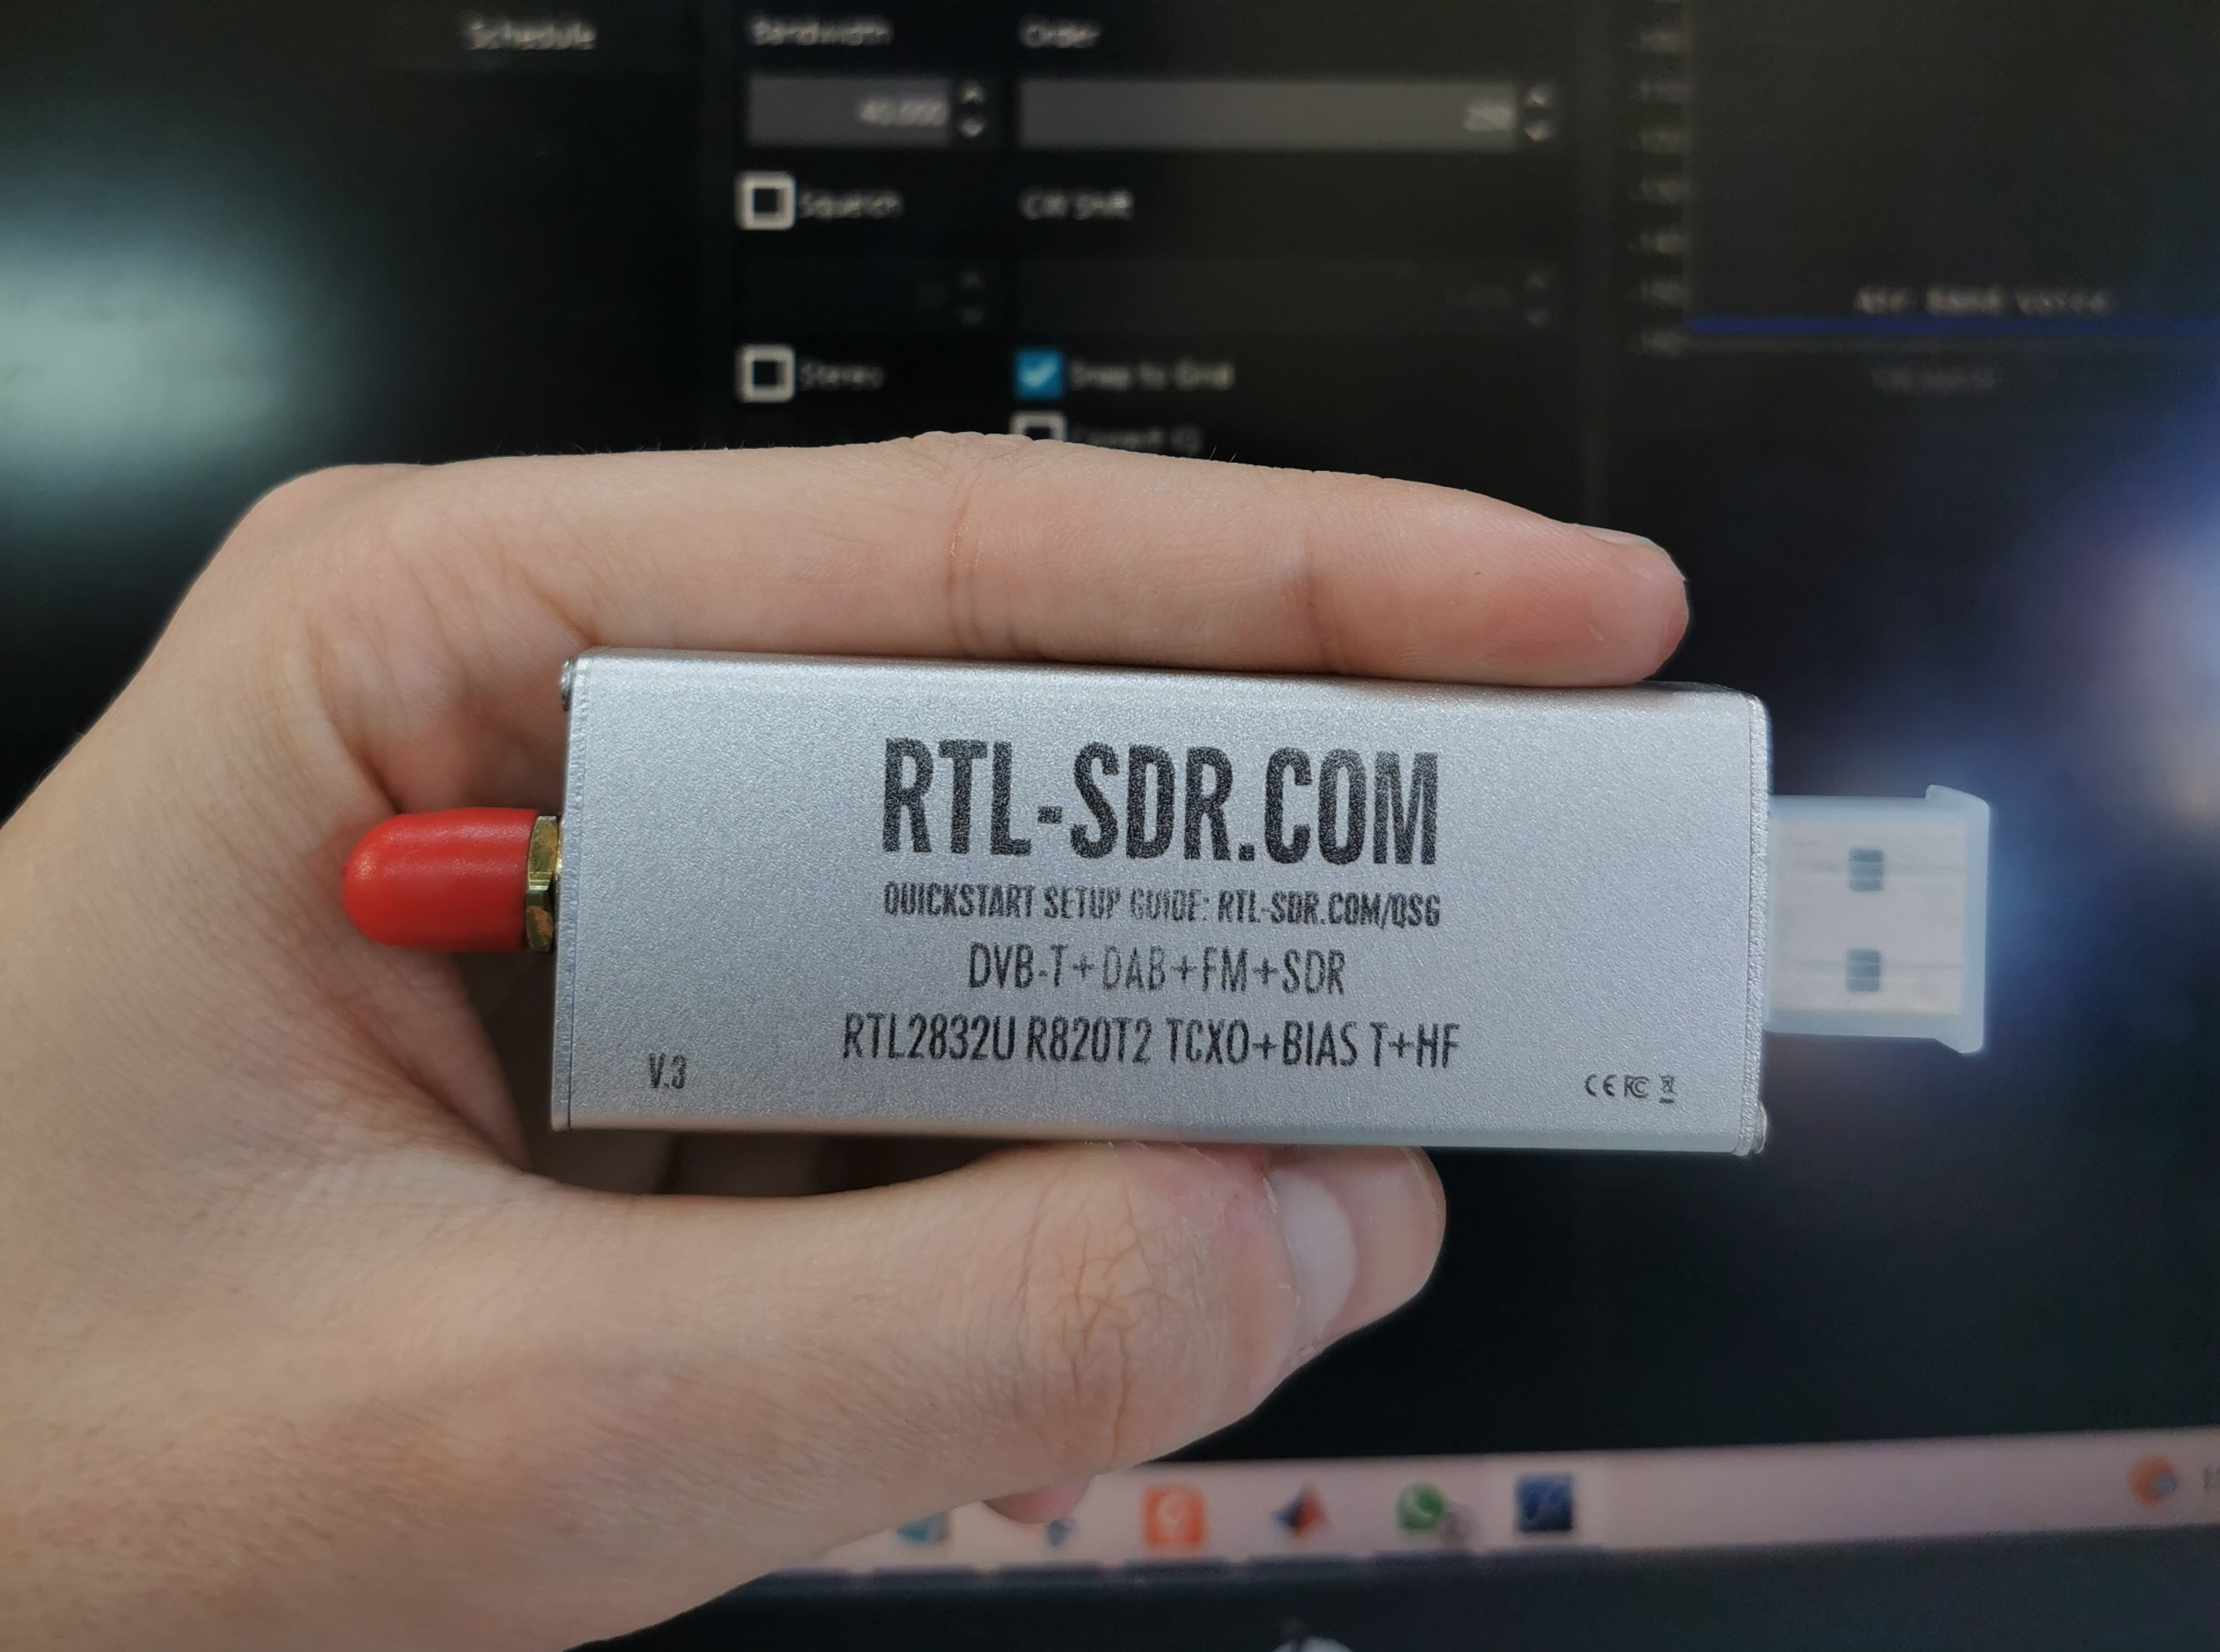
\includegraphics[width=\textwidth, height=5cm]{imagenes/rtl.JPG}
    \caption{RTL-SDR utilizado}
    \label{rtl}
  \end{subfigure}
  \caption{Esquema RTL-SDR}
\end{figure}

Este tipo de dispositivos fueron pensados primeramente como receptores DVB-T para la televisión, pero su gran versatilidad ha dado lugar a diferentes usos en FM, AM e incluso GPS.
El RTL-SDR utilizado en el proyecto se muestra en la Figura [\ref{rtl}] y su interior en la Figura [\ref{inner_RTL}].
\newpage
\section{Software}

	\subsection{Programa Gpredict}
	Se ha utilizado como herramienta de apoyo el programa \textit{Gpredict}. Es un programa que llega a proporcionar información sobre una gran cantidad de satélites, así como su órbita, velocidad y frecuencia a la que emiten, tiempo en función de la posición...
	
	Es necesario definir primero una estación baso. En el caso de este proyecto, se han definido las coordenadas de Granada, España. Una vez definida la estación base, se seleccionan los satélites a los que les quieres realizar el seguimiento. En este caso serán los satélites NOAA activos (NOAA-18, NOAA-19 y NOAA-15). La interfaz del programa con la estación base y los satélites definidos se muestra en la Figura [\ref{gpredict}].
	
	\begin{figure}[H]
 \centering
 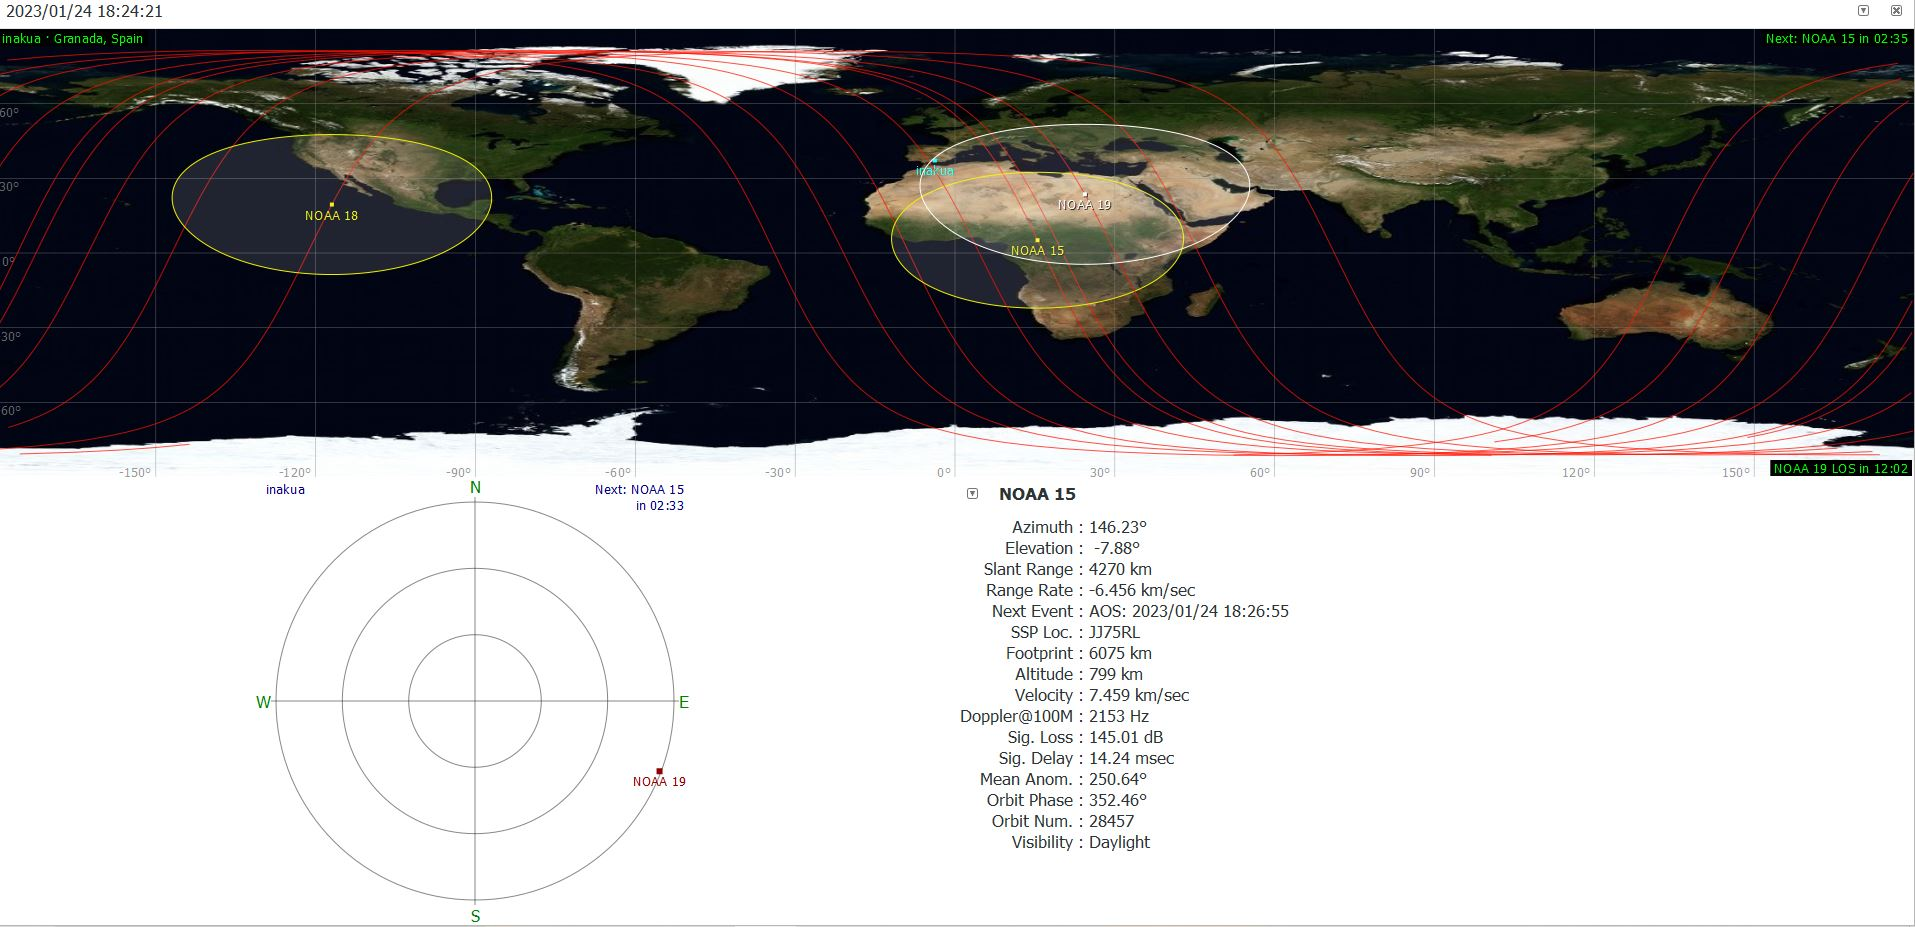
\includegraphics[width = 1 \linewidth]{imagenes/Gpredict_NOAA.JPG}
 \caption{Gpredict satélites NOAA}
 \label{gpredict}
 \end{figure}
 
 En la parte inferior de la captura de pantalla se puede visualizar la posición en coordenadas del satélite y otros datos como la velocidad, altitud, fase, elevación y hasta una aproximación del efecto Doppler en unidades de frecuencia.
 
 Más información sobre cada satélite se puede consultar mediante click derecho en el satélite en cuestión. Es de interés la información de \textit{Future Passes}, la cual ayuda a saber a qué momento del día va a pasar el satélite cerca de nuestra ubicación de la estación base.
 
   Dentro de esta misma opción, se puede visualizar gráficamente la trayectoria del satélite, como se observa en la Figura [\ref{trayectoria}]. Esta representación es de gran ayuda para saber el tiempo óptimo a la hora de captar la señal. Con los datos proporcionados por \textit{Gpredict}, se ha logrado en este proyecto captar las señales de los satélites NOAA para los tiempos previstos, por lo que es de gran utilidad.

	\begin{figure}[H]
 \centering
 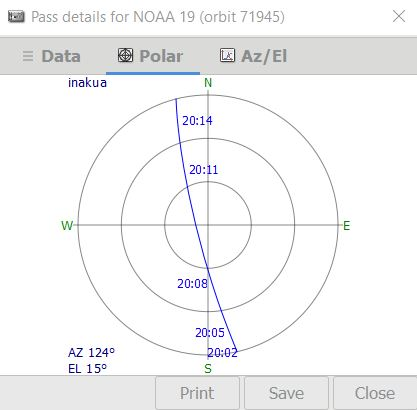
\includegraphics[width = 9cm]{imagenes/future_passes.JPG}
 \caption{Trayectoria NOAA-19}
 \label{trayectoria}
 \end{figure}
 

	\subsection{Diagrama de flujo en GNU Radio}
	Con el propósito de procesar la señal recibida del RTL-SDR a tiempo real se ha creado un diagrama de bloques en GNU Radio. Los pasos a realizar en el procesamiento de la señal se han realizado teniendo en cuenta el estándar APT y son los siguientes:
	\begin{enumerate}
	\item Filtrado paso baja y decimado
	
		\begin{figure}[hbtp]
 \centering
 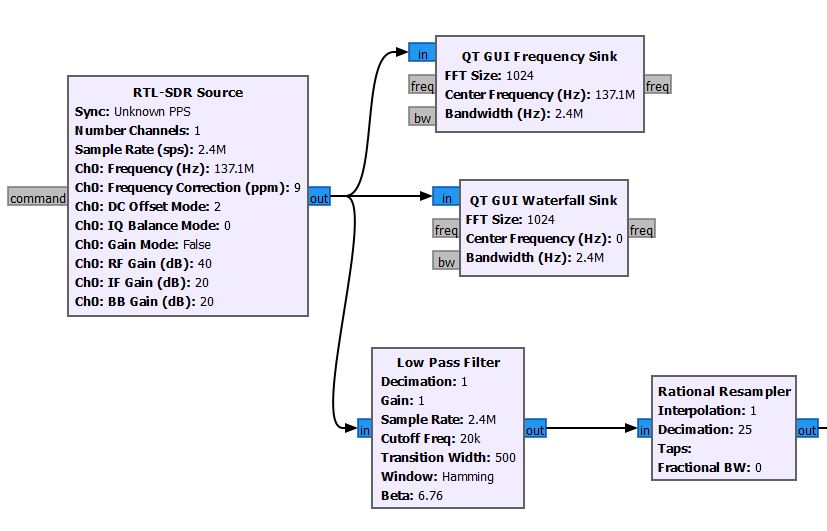
\includegraphics[width = 12cm]{imagenes/primer_paso.JPG}
 \caption{Filtrado y decimado}
 \label{filtardo_decimado}
 \end{figure}
 
 El bloque de ''RTL-SDR Source'' capta la señal directamente del dispositivo, con una tasa de muestreo de $2.4 MHz$, la frecuencia central la del satélite deseado y una ganancia en RF bastante alta (unos 35-40 dB).
 Se filtra paso baja con una frecuencia de corte poco restrictiva de $20 kHz$ para eliminar contribuciones ruidosas, ya que debido al efecto doppler, la frecuencia central de la señal del satélite podría variar y si se posee un ancho de banda restrictivo parte de la información podría perderse. Posteriormente se remuestrea la señal para trabajar a $96 kHz$.

Los bloques restantes no mencionados corresponden a \textit{GUI}, es decir, el espectro de la señal mostrado por pantalla.
 
 
 
	\item Demodulación FM
	
		\begin{figure}[hbtp]
 \centering
 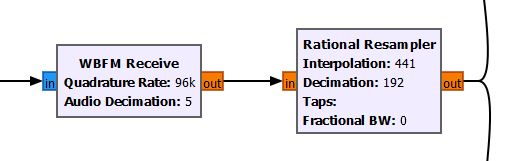
\includegraphics[width = 12cm]{imagenes/wbfm.JPG}
 \caption{Demodulación FM}
 \label{wbfm}
 \end{figure}
 
 Para demodular en FM simplemente se ha utilizado el bloque \textit{WBFM} el cual demodula la señal FM de banda ancha de entrada. Una vez con la señal demodulada, se adapta la frecuencia de muestreo a una típica de audio.	
	
	\item Demodulación AM y construcción de la imagen
	
		\begin{figure}[hbtp]
 \centering
 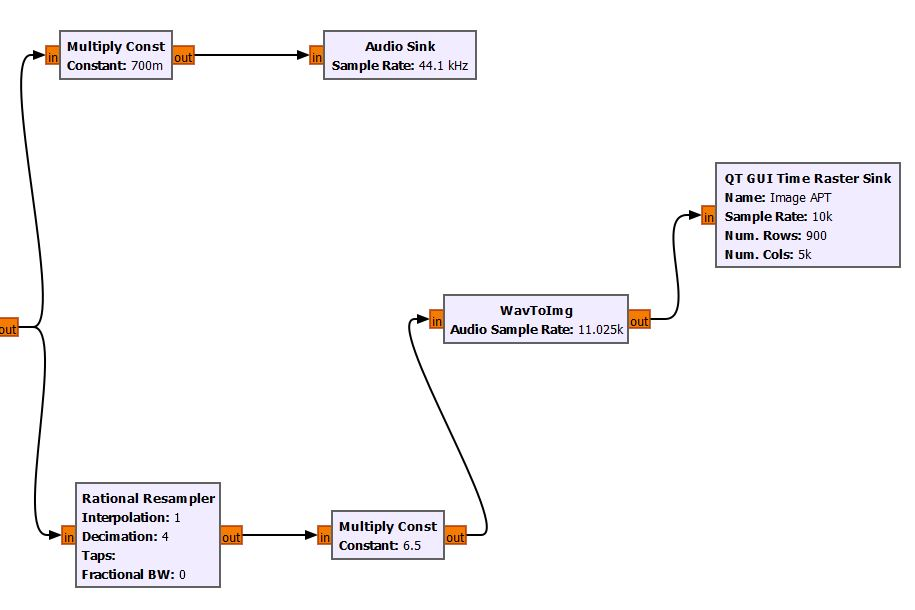
\includegraphics[width = 12cm]{imagenes/apt_blocks.JPG}
 \caption{Demodulación AM}
 \label{apt_blocks}
 \end{figure}
	
	
Después de obtener la señal de audio a la frecuencia de $11.025 kHz$, se llega a un bloque jerárquico llamado \textit{WavToImg} el cual realiza la correspondiente conversión de señal de audio a imagen APT. El interior de este bloque se muestra en la Figura [\ref{wavtoimage}].

 \begin{figure}[H]
 \centering
 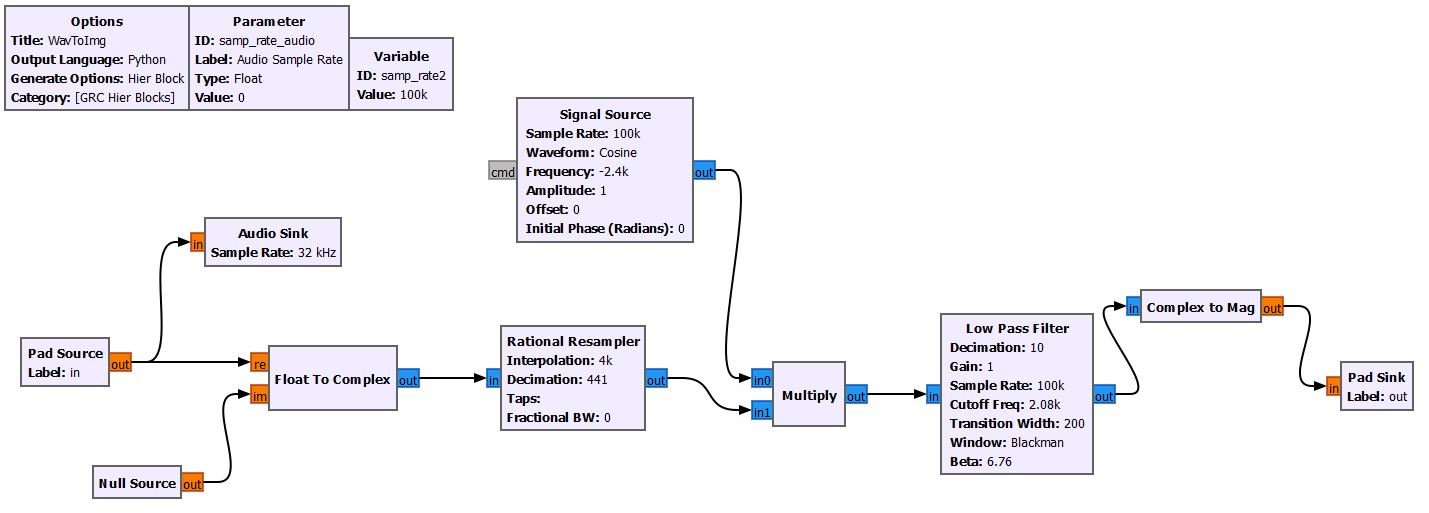
\includegraphics[width = 1 \linewidth]{imagenes/APT_hier.JPG}
 \caption{Bloque WavToImg}
 \label{wavtoimage}
 \end{figure}	
 
 El procedimiento se basa en una demodulación AM teniendo en cuenta que la información APT de interés se encuentra en una subportadora de $2.4 kHz$. 
	Según el estándar, se recomienda hacer un remuestreo a una frecuencias e $100 kHz$ antes de hacer la demodulación. Para llevar la subportadora a banda base se ha utilizado un coseno a una frecuencia de $-2.4 kHz$ y se ha hecho un filtrado posterior.
	
La salida del bloque "WavtoImg" proporciona la señal APT demodulada y se muestra la imagen por pantalla a tiempo real.
	
	
	\end{enumerate}
	
	 En la \textit{Figura \ref{diagrama_completo}} se aprecia el diagrama de flujo completo.
	
	\begin{figure}[hbtp]
 \centering
 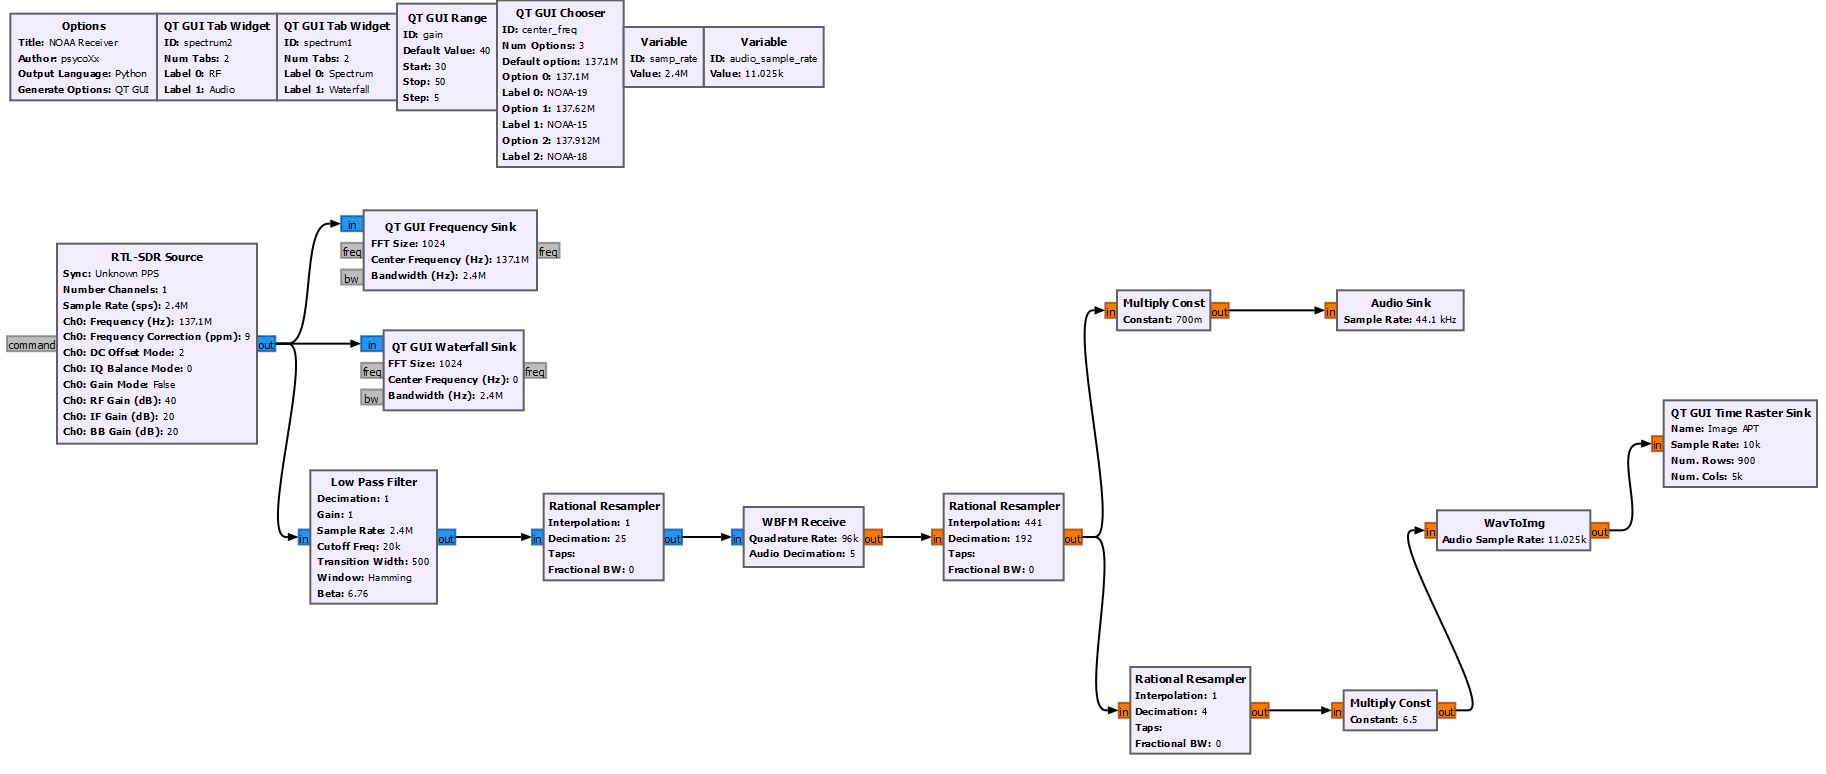
\includegraphics[width = 1 \linewidth]{imagenes/diagrama_flujo_completo.JPG}
 \caption{Diagrama de flujo}
 \label{diagrama_completo}
 \end{figure}

\newpage


	\subsection{Corrección del efecto Doppler}

	Para la corrección del efecto Doppler que afecta a la imagen se pueden llevar a cabo dos aproximaciones distintas: en tiempo real y a posteriori:
	
	\begin{itemize}
	
	\item \textbf{En tiempo real:} Para realizar una corrección en tiempo real del efecto Doppler se debe contar con información en tiempo real de la órbita del satélite. Conociendo su posición, dirección y velocidad (así como la posición del receptor, asumiéndolo estático) se puede obtener fácilmente la variación de frecuencia causada por el efecto Doppler. El único problema de esta aproximación es que se tienen que exportar en tiempo real los datos de la órbita de una aplicación de observación a la aplicación que se utilice para el procesamiento de la señal. Considerábamos que esta opción no era la idónea, por lo que nos centramos en una aproximación a posteriori.
	
	\item \textbf{A posteriori:} Bajo este esquema, se obtiene una señal afectada por el efecto Doppler, y se le aplica un algoritmo que elimina dicho efecto. Este ha sido el método elegido para este proyecto.
	
	\subsection{Método propuesto} 
	
	Utilizando un método a posteriori, se puede corregir el efecto Doppler de cualquier imagen APT, con independencia del momento en el que se tomó la imagen y sin necesidad de contar con la información exacta de la órbita del satélite en el momento de paso. Se ha implementado un algoritmo en Matlab, basando su fundamento en \cite{7}, que lleva a cabo una corrección. Su funcionamiento está basado en la interpolación / decimado de las líneas de la imagen, en base a la información aportada por el estándar APT. El algoritmo parte de la señal AM, ya que la demodulación FM se realiza automáticamente en la aplicación de captura. La descripción del algoritmo:

\begin{itemize}

	\item Se realiza un filtrado de la señal AM para eliminar posibles componentes indeseadas. La señal se sobremuestrea para que la corrección del efecto Doppler pueda realizarse con una precisión 'sub-píxel' lo que nos dará los mejores resultados.
	
	\item Se crea el pulso de sincronización del primer canal de la imagen, con el que se practica la correlación con la señal recibida. El resultado de esta función de correlación nos dará una serie de picos que nos indicarán el comienzo de cada línea.
	
	\item Se analiza cada línea en un bucle, en la que se compara la longitud real de cada línea con la longitud que debería tener de acuerdo con el estándar (2080 píxeles). Si la longitud es la esperada no se realiza ninguna operación, si la longitud es menor o mayor de la esperada, se practica una interpolación o un decimado, respectivamente. Con este método, todas las longitudes de las líneas pasan a ser iguales, con un comienzo y un final equivalente. De esta manera se elimina el efecto sobre la imagen del efecto Doppler. La imagen se decima a su tamaño original y se representa.
	




\end{itemize}
	

	
	
	\end{itemize}

\newpage

\section{Resultados}

La implementación del método propuesto fue exitosa. Se consiguió demodular la información contenida en la imagen AM, así como corregir el efecto Doppler de la imagen de manera exitosa. Como referencia, se muestra a continuación la representación de la imagen tras la demodulación AM, sin utilizar los pulsos de sincronización y sin realizar la corrección del efecto Doppler:


 \begin{figure}[H]
 \centering
 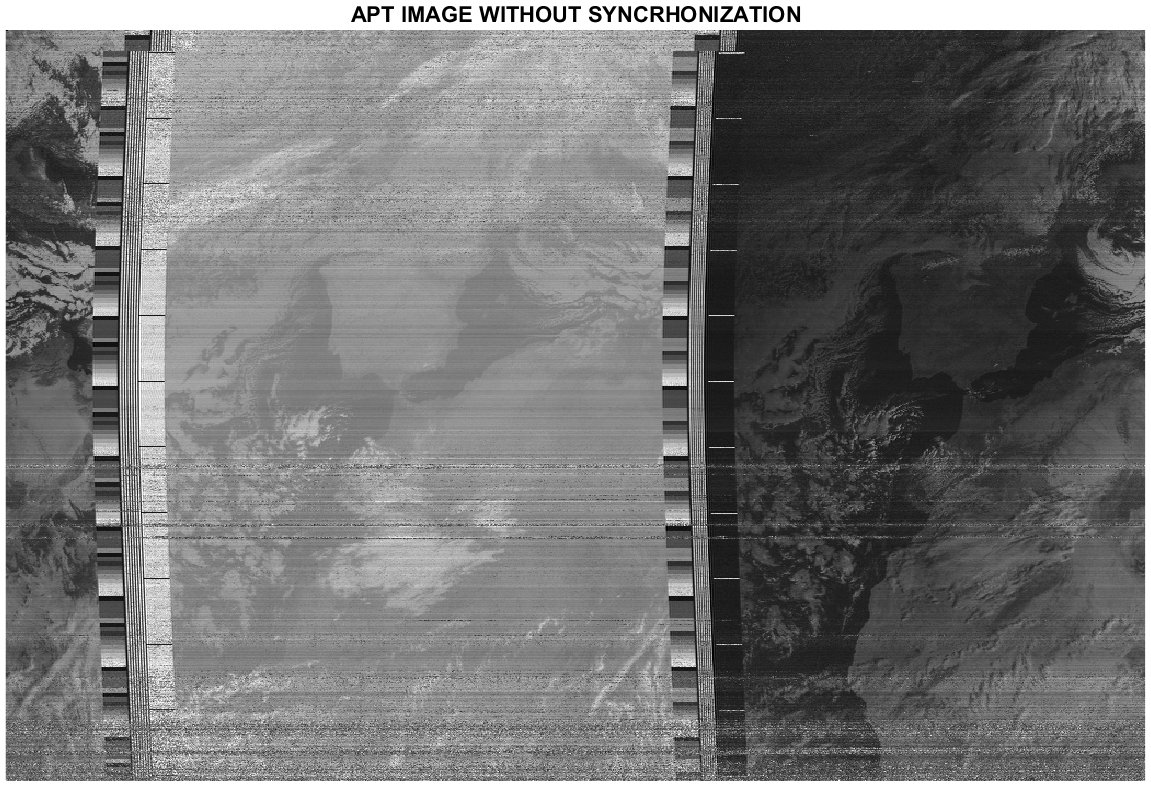
\includegraphics[width = 13cm]{imagenes/31_01_nosynch.png}
 \caption{Representación de la imagen sin corrección del Efecto Doppler}
 \label{apt_nosynch}
 \end{figure}
 
 Tras aplicarle a la imagen el algoritmo descrito en el apartado anterior, se consigue una corrección total del Efecto Doppler, así como un ajuste de la imagen al estándar APT, gracias a los pulsos de sincronización:

 \begin{figure}[H]
 \centering
 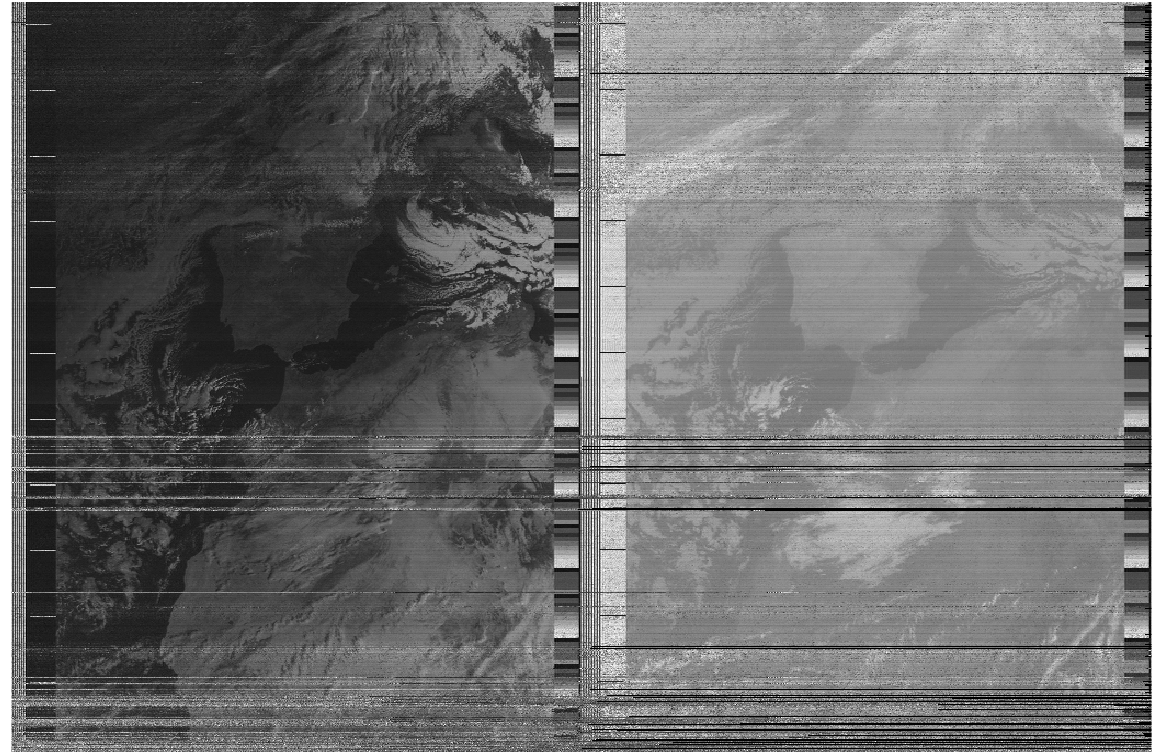
\includegraphics[width = 13cm]{imagenes/31_01_synch.png}
 \caption{Representación de la imagen con corrección del Efecto Doppler}
 \label{apt_corrected}
 \end{figure}
 
 Como se puede comprobar, las consecuencias del efecto Doppler han desaparecido por completo, y se consigue un ajuste conforme a lo que estipula el estándar en \ref{APT_FRAME}. Las líneas que no se han obtenido correctamente, se deben a errores en la antena o a una distancia excesiva entre satélite-receptor (cuando el satélite se encontraba cerca del horizonte la potencia recibida era mínima). Para la obtención de la señal con una SNR correcta con la antena diseñada, se debía mantener en todo momento una orientación adecuada a la zona de paso del satélite. Mantener esta orientación en todo momento resulta complicado, y da como resultado la pérdida de ciertas líneas. Al perder la situación del pulso de sincronización en   dichas líneas tiene como consecuencia la pérdida total de información de esa línea, ya que el algoritmo desconoce qué información corresponde a esa línea. La señal que se ve plasmada en las imágenes se obtuvo en una pasada del satélite NOAA-19. Como aspecto adicional, en la Figura [\ref{perfil-pasada}] se muestra el perfil de pasada del satélite. Como se puede comprobar, las condiciones eran bastante buenas, puesto que cuanto más cercano sea el paso con respecto a la  vertical del receptor, mayor será la potencia recibida.
 
  \begin{figure}[hbtp]
 \centering
 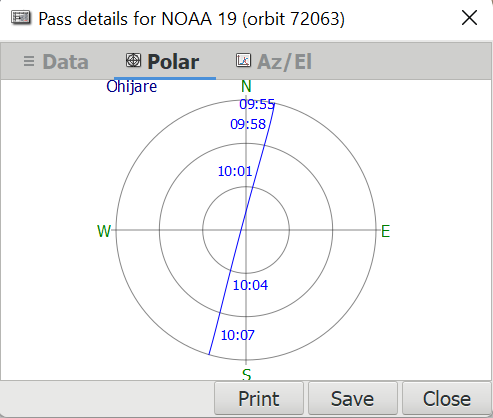
\includegraphics[width = 10cm]{imagenes/noaa_19 pass 31_01.png}
 \caption{Perfil de pasada NOAA-19}
 \label{perfil-pasada}
 \end{figure}
 
 
 

 

\section{Dificultades en la realización del proyecto}

Durante la realización del proyecto se han enfrentado diversas dificultades que se detallan a continuación:
\begin{itemize}

    \item \textbf{GNU-Radio y SDR}: Pese a que conocíamos ambas tecnologías, no habíamos desarrollado ningún proyecto utilizándolas y familiarizarnos con ellas requirió tiempo.
    \item \textbf{Diseño y montaje de la antena}: Tal y como se ha desarrollado anteriormente, la elección de la antena no fue una tarea fácil y aún menos lo fue el montaje. Tuvimos varios problemas a la hora de construirla:
    \begin{itemize}
        \item Montaje inical de la antena. El proceso de conexión del cable coaxial a la antena en una disposición lo suficientemente robusta, así como el montaje del adaptador SMA se demostró un proceso más tedioso y complicado de lo que se pensó inicialmente. Se tuvieron que realizar soldaduras y reconstrucciones que no estaban en la planificación inicial del proyecto.
        \item Rotura del montaje: la antena sufrió un pequeño accidente que hizo que tuvierámos que volver a conectar el cable coaxial a un nuevo SMA del que en aquel momento no se disponía.
    \end{itemize}
    \item \textbf{Recepción y procesamiento de las señales}: Obtener una señal con la calidad suficiente, fue un proceso que tuvo cierta curva de aprendizaje, ya que tuvimos numerosos intentos fallidos hasta que pudimos conseguir la configuración adecuada en recepción, así como la orientación y posición geográfica adecuada. Entre los muchos factores que influyeron el proceso de recepción se destacan:
    \begin{itemize}
    		\item Posición geográfica: Los primeros intentos de obtención de señal se hicieron en un lugar cercano a una casa, que, aunque con vistas prácticamente completas al cielo, no dio los resultados esperados. Acusamos estos errores a las posibles reflexiones que podían ocurrir con los edificios cercanos, así como la pérdida momentánea de LOS por obstáculos intermedios. Al cambiar la posición a un descampado sin edificios en decenas de metros de distancia, los resultados mejoraron notablemente.
        \item Orientación de la antena: La antena ha de tener una orientación concreta con respecto al satélite en cada caso. Bajo nuestra experiencia comprobamos que no se podía mantener estática si se quería obtener correctamente la imagen. 
        \item Tiempo de medida: Por cada medida se requieren de media unos 10 min en los que la orientación debe ser correcta y no debe haber obstáculo alguno entre satélite-receptor.
        \item No siempre existe LOS.
        \item Configuración de SharpSDR: El ancho de banda de recepción era de extremada importancia para la obtención de una señal clara y sin ruido, debía ser lo más ajustada posible al ancho de banda original de la señal. Esto no era posible, ya que debido al efecto Doppler la frecuencia aparente iba desplazándose conforme el paso del satélite, y se podía llegar a perder información. Se llegó a un compromiso que llevó varios intentos hasta que se llegó al adecuado.
    \end{itemize}
    
\end{itemize}

\newpage
\section{Conclusión}

\subsection{Conclusiones}
Este proyecto se ha realizado durante dos meses y con una disponibilidad temporal de los integrantes limitada. A pesar de ello, se ha logrado avanzar relativamente rápido y se han logrado unos buenos resultados. Ha sido un proyecto con poco presupuesto, por lo que, seguramente, invirtiendo en una antena con mejores prestaciones o la incorporación de un empotrado hubiera mejorado notablemente los resultados.
Ha sido un proyecto bastante completo, ya que se ha profundizado en diseño de antenas, a la hora de construir la antena de tipo dipolo en V y en el procesado de señal con la parte de radio definida por software. Además, los objetivos iniciales del proyecto se han abarcado sin problemas, ya que se ha logrado captar correctamente múltiples señales de satélites NOAA convirtiendo estas a imágenes perfectamente visibles, consiguiendo una corrección del efecto Doppler muy precisa.

\subsection{Líneas Futuras}

Como futuras mejoras, se propone la construcción de una antena con polarización circular, ya que esta es independiente de la orientación y no haría falta un factor externo para optimizar la captación de la señal a medida que el satélite se desplaza. 
Otra mejora sería la inclusión de un sistema empotrado conectado al RTL-SDR. De esta manera, mediante alguna orden externa, se podría captar la señal sin la necesidad de tener conectado un hardware como puede ser el ordenador. A nivel de hardware, la inclusión de un LNA (Low Noise Amplifier) sería interesante de cara a obtener la señal con mejores prestaciones.
Respecto a la corrección del efecto doppler, se ha propuesto una vía alternativa mediante la interpolación-decimado, el cual no depende de datos como la velocidad del satélite. Sin embargo, esta corrección que se ha realizado se realiza de forma asíncrona, por lo que una nueva mejora sería implementar una corrección del efecto doppler a tiempo real. De esta nueva forma serán necesarios datos como la velocidad del satélite en todo momento y la debida conexión a un software de seguimiento de satélites a tiempo real como puede ser \textit{Gpredict}.
La resolución de las imágenes obtenidas es limitada, debido a que en un estándar analógico como APT, la calidad máxima no es tan alta como la común a día de hoy, en el que cientos de satélites envían imágenes a color en alta resolución. Una vía de mejora podría consistir en la obtención de imágenes enviadas en formato digital de un satélite de meteorología, como la serie de satélites rusos METEOR-M2. Estas imágenes se pueden obtener de una manera relativamente similar, proporcionando una imagen a color y de mucha mayor resolución.

\newpage

\section{Presupuesto}
Una vez completado el proyecto, el presupuesto asociado al mismo se detalla en la Tabla [\ref{Tab3:Presupuesto}].

\begin{table}[h!]
\centering
\begin{tabular}{|c|c|c|} 
\hline
\textbf{Material}          & \textbf{Unidades} & \textbf{Coste/Unidad}            \\ 
\hline
\textbf{Aluminio}          & 2m                & 0.81\euro{}/m   \\ 
\hline
\textbf{Juntas}            & 1                 & 0.30\euro{}     \\ 
\hline
\textbf{Estructura Antena} & 1                 & 5\euro{}        \\ 
\hline
\textbf{SDR}               & 1                 & 45.98\euro{}    \\ 
\hline
\textbf{Conectores SMA}    & 10                & 1.1\euro{}/SMA  \\ 
\hline
\textbf{Cable Coaxial}     & 3m                & 1.2\euro{}/m    \\ 
\hline
\textbf{Ordenador}               & 1                 & 800\euro{}    \\ 
\hline
\multicolumn{2}{|c|}{\textbf{Coste total}}              & 867.49\euro{}    \\
\hline

\end{tabular}
\caption{Tabla resumen del presupuesto del proyecto.}
\label{Tab3:Presupuesto}
\end{table}

\newpage

\begin{thebibliography}{11}


\bibitem{1}137 MHz WX-SAT original 9A4QV V-dipole antenna. (2020, December 28).

\bibitem{2}Automatic Picture Transmission (APT). (n.d.). Sigidwiki.com. Retrieved January 31, 2023, from https://www.sigidwiki.com/wiki/Automatic-Picture-Transmission-(APT)

\bibitem{3}Crisan, N., Cremene, L. (n.d.). Noaa signal decoding and image processing using gnu-radio. Utcluj.Ro. Retrieved January 31, 2023

\bibitem{4}gr-gpredict-doppler: GNU Radio Gpredict Doppler shift correction block. (n.d.).

\bibitem{5}How it works. (n.d.). Com.Ar. Retrieved January 31, 2023, from https://noaa-apt.mbernardi.com.ar/how-it-works.html

\bibitem{6}How to build A V Dipole for receiving weather satellites. (2020, May 31).

\bibitem{7}Lin, S.-S., Song, Y.-Z. (2021). A Doppler effect correction method for APT weather satellite image reception. 2021 International Symposium on Intelligent Signal Processing and Communication Systems (ISPACS).

\bibitem{8}NOAA-19 APT reception using GNU radio and a FUNcube dongle. (n.d.). Websterling.com. Retrieved January 31, 2023, from http://websterling.com/tsro/apt/

\bibitem{9}RTL-SDR tutorial: Receiving NOAA weather satellite images. (2013, May 13). Rtl-sdr.com. https://www.rtl-sdr.com/rtl-sdr-tutorial-receiving-noaa-weather-satellite-images/


\bibitem{10}Simple NOAA/Meteor weather satellite antenna: A 137 MHz V-dipole. (2017, March 1). Rtl-sdr.com. https://www.rtl-sdr.com/simple-noaameteor-weather-satellite-antenna-137-mhz-v-dipole/


\bibitem{11}Table of contents. (1989). Space Science Reviews, 50(3–4). https://doi.org/10.1007/bf00228384


\end{thebibliography}



\end{document}
